\todo {Make it clear that the goal of this work is continuous sensing}
\todo{Explain that we approach continuous sensing on two stages: 1) continuous availability and 2) randomized response}
\begin{figure}
	\centering
%	\begin{subfigure}{\columnwidth}
%		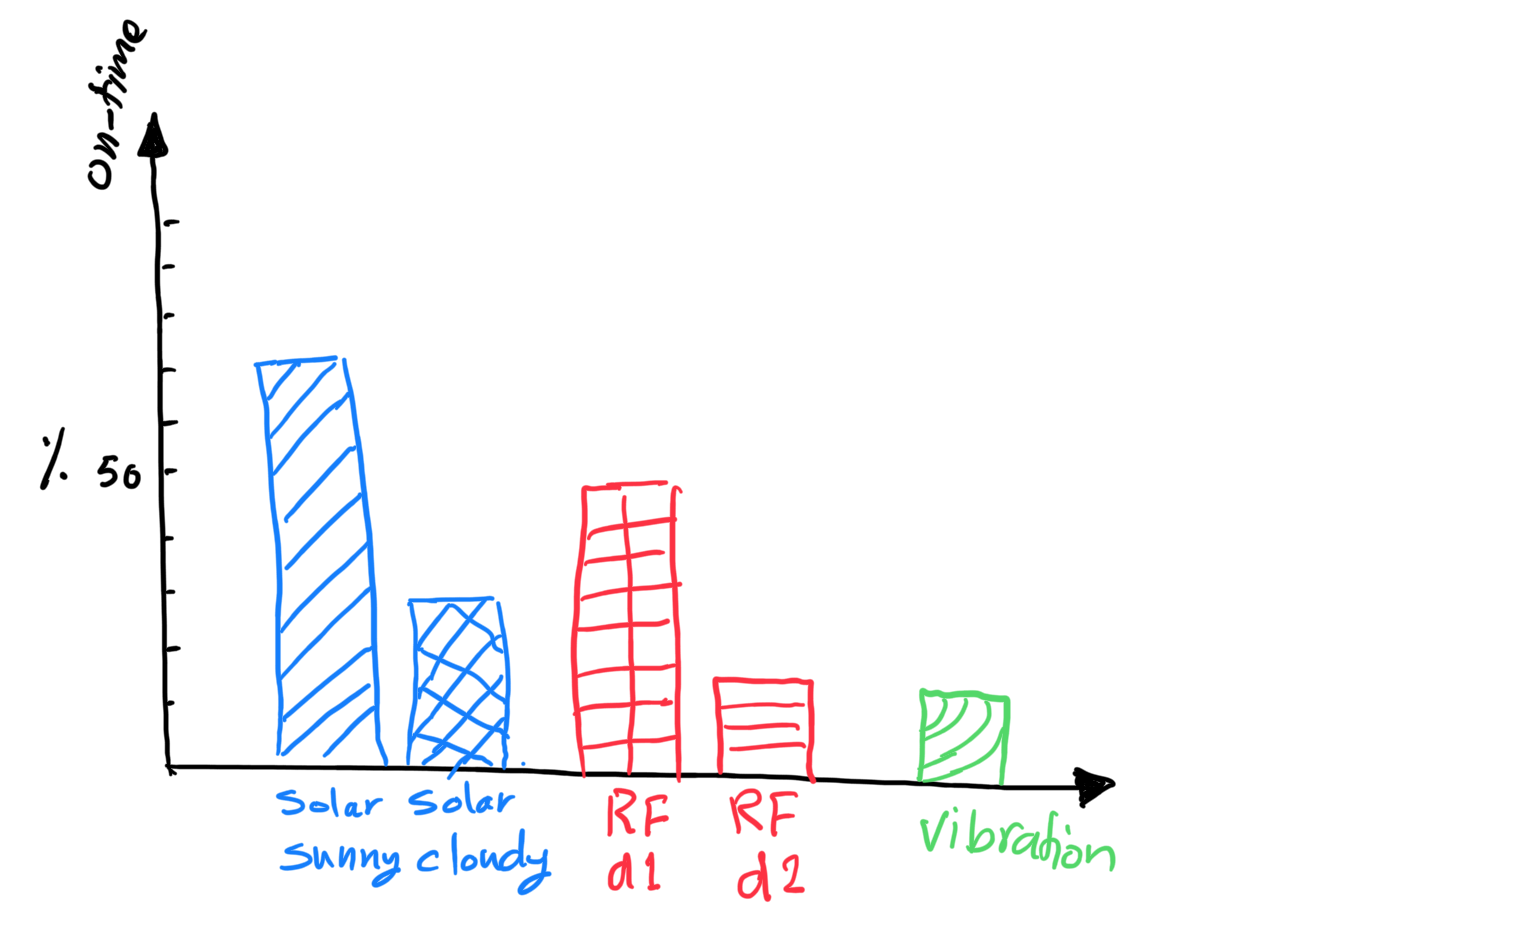
\includegraphics[width=\columnwidth]{figures/intermittent_problem}
%		\caption{The up time percentage of an intermittent device powered by different energy sources relative to its on/off cycle length}
%		\label{fig:disInterSys}
%	\end{subfigure}
%	\begin{subfigure}{\columnwidth}
		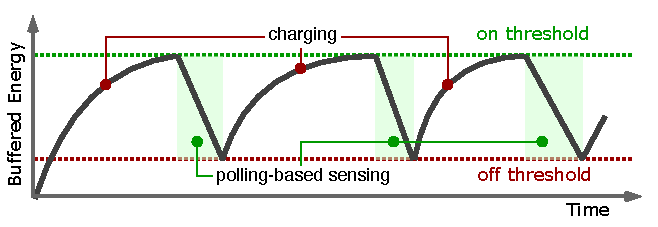
\includegraphics[width=\columnwidth]{figures/PowerCycleIntermittentSystem}
		\caption{The power cycle of an intermittently powered device.}
		\label{fig:powerCycle}
%	\end{subfigure}
\end{figure}

The Internet of Things is the engine that will drive smart cities. In these cities, cars will not need to wait in front of traffic lights for non-existing pedestrians to cross the road; doors, upon leaving, will provide people with weather forecast; and jackets will adjust air circulation based on body temperature. Smart cities will gain their awareness through billions of sensors.

Battery-powered sensors do not provide a viable solution to power all the sensors in smart cities. Batteries require (i) regular maintenance, even rechargeable ones wear out in a few years \cite{xxx}; and (ii) hazard waste management. Moreover, the batteries raw materials are also limited. The edges of the future Internet of Things must leave batteries behind and rely on perpetual energy sources. 

Natural energy sources such as light, vibration, and heat can power these sensors directly. Tiny energy harvesters, however, can only scavenge a very limited power from such energy sources. Therefore, an energy-harvesting sensor operate intermittently. An intermittent sensor starts by harvesting a certain amount of energy in its buffer (i.e. a super-capacitor). Then, it triggers operation which depletes the buffered energy quickly, as the power consumption rate tends to be much higher than the power accumulation rate. Once the energy is below a certain level, the sensor experience a complete power-down and the harvester starts accumulating energy again (Figure~\ref{fig:powerCycle}). Intermittent nodes trade-off reliability (reliable energy source) for sustainability (sustainable energy source for a very large number of sensory nodes). This trade-off generates many challenges. For example, preserving forward computation progress, enabling timely operations, and the fact that nodes are not always available. 

%Energy harvesters are a promising battery replacement, scavenging power from ambient sources instead of fixed reservoirs. A tiny energy harvester, however, powers a device intermittently: it accumulates energy in its buffer (i.e. super-capacitor) until a threshold is reached, and then it powers the sensors which depletes the energy reservoir and terminates execution. 

Many intermittent power-supply related problems have been addressed. For example, intermittent computation problem, which is concerned with the preservation of an application progress and memory integrity under frequent power failures~\cite{mementos,dino,colin2016chain}; timely operation, which is concerned with data freshness after a power interrupt; event-driven execution, which is concerned with I/O operations under arbitrarily-timed power loss. However, all previous work has considered the intermittency as an inherent characteristic of these systems and have not attempted to control it \todo{make it clear that intermittency is a random process}.  

Despite the significant progress that has been achieved in the intermittent domain, the system availability problem has not been addressed. With arbitrarily timed and time-spanned power-ups, intermittently-powered sensors do not meet the requirements of a wide spectrum of real-world applications. Consequently, they have not gained widespread adaptation. This paper tackles the paradox of continuous sensing on intermittent devices by introducing a new type of sensors that we call \textit{\fullsys} (\sys). The \sys is defined as a group of intermittent nodes with randomized on/off cycles. \sys distinguishes between different energy conditions and adapts its response accordingly to efficiently distribute its resources and to approach continuous sensing.  

We put our observations and theory into test by realizing a \sys instant in the form of distributed intermittent voice assistant agent. We tested the voice assistant in different energy conditions and the results validate our assumptions and observations. 

Highlights of the paper contributions:
\begin{itemize}
		\item Introducing a new sensor type: \textit{\fullsys} (\sys) is a group of intermittently powered nodes that takes advantage of the randomized nature of the powering subsystem (energy source and energy harvester) to approach 100\% system availability. \sys has a sensing algorithm that is energy harvesting conditions aware and therefore it is an efficient sensor. 
		\item Characterizing the behavior of coalesced intermittent sensor under different energy conditions.
		\item Characterizing the behavior of coalesced intermittent sensor under different event occurrence frequencies and patterns. 
		\item Implement a coalesced intermittent sensor in the form of a distributed intermittent microphone array. 
\end{itemize}





\todo{to be removed!}
%
%%% Hypothesis, question, purpose statement
 It increases the temporal and spatial availability of an intermittent system and enables resource distribution such as large number of words templates for spoken words recognition systems. 

Controlling the on/off cycle of intermittent devices enables adapting them to many real world applications. For example, once a certain on/off cycle is preserved, an intermittent wake-up receiver can be implemented; intermittent acoustic monitoring system for monitoring engines modules---the sound produced by a deformed gear tooth---can be made. Moreover, with the advances in passive communication (such as passive light~\cite{}, and backscatter tag-to-tag~\cite{} communication) battery-free miniaturized sensors can form self-powered wireless sensor network to, for instance, create smart wallpaper and revolutionize smart buildings. 


